\title{LEZIONE 18 9/04/2020}\newline
\textbf{link} \href{https://web.microsoftstream.com/video/a6351498-1edd-4ec9-b134-3b5fd7a9a3ee?list=user&userId=faa91214-a6f5-40d7-8875-253fd49b8ce1}{clicca qui}
\section{Schema fondamentale di un anello di controllo (SD LTI a TC, SISO)}
\subsection{Schema completo}
[immagine dagli appunti del prof]
\begin{center}
    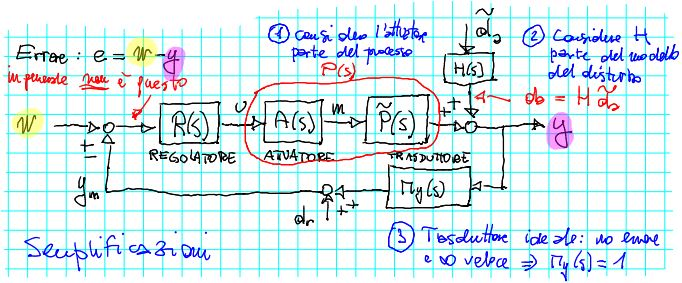
\includegraphics[height=5cm]{../lezione18/img1.JPG}
\end{center}
Ogni blocco rappresenta una funzione di trasferimento e prendiamo come presupposto che tutti i blocchi singoli blocchi non abbiano parti nascoste, anche se il complessivo potrebbe averne.\newline
\newline
$\tilde{P}(s)$ prende il nome di \textbf{processo}. La funzione di trasferimento $A(s)$ prende il nome di \textbf{attuatore} che ha in ingresso il segnale di controllo $u$ e che in base ad esso invia al processo un segnale $m$.\newline
\newline
Abbiamo poi il \textbf{regolatore} (o controllore) $R(s)$. Prima del regolatore è presente un \textbf{nodo formatore} (o comparatore) che prende in ingresso il \textbf{segnale di riferimento} $w$ (output desiderato).\newline
\newline
Dopo il processo è presente un nodo sommatore che aggiunge un \textbf{disturbo} esterno $\tilde{d}_a$ che segue la sua dinamica $H(s)$.\newline
\newline
Infine abbiamo il blocco $M_y(s)$, che prende il nome di \textbf{trasduttore}. A sua volta il traduttore ha dei disturbi esterni che indichiamo con $d_r$ e solo ora abbiamo la \textbf{variabile controllata} $y_m$.\newline
\newline
Definiamo ora l'\textbf{errore} come $w-y$, che in generale non è il segnale in ingresso nel regolatore, in quanto non lavoriamo con la quantità $y$, ma con la misurazione $y_m$.
\subsection{Schema semplificato}
Facciamo delle semplificazioni di questo schema:
\begin{itemize}
    \item consideriamo l'attuatore parte del processo: $P(s)$ è la serie di $A(s)$ e $\tilde{P}(s)$;
    \item consideriamo $H$ parte del modello del disturbo: $d_a = H \tilde{d}_a$;
    \item consideriamo un trasfuttore ideale: non c'è errore ed è infinitamente veloce, $M_y(s) = 1$.
\end{itemize}
Quindi lo schema semplificato che useremo sarà così:\newline
[immagine dagli appunti del prof]
\begin{center}
    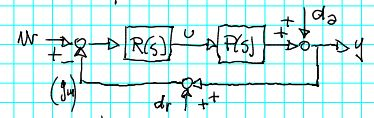
\includegraphics[height=3cm]{../lezione18/img2.JPG}
\end{center}
\textbf{oss.} $d_a$ fa raramente cambiare $y$, $d_r$ no, si limita a corromperne la misura.\newline
\newline
In questo schema semplificato le funzioni di trasferimento di interesse sono:
\begin{itemize}
    \item $L(s) = R(s)P(s)$ che è la funzione di trasferimento di anello (aperto);
    \item $S(s) = \frac{1}{1+L(s)}$, che prende il nome di \textbf{funzione di sensitività}, notiamo che $S= \frac{Y}{D_a}$;
    \item $T(s) = \frac{L(s)}{1+L(s)}$, che prende il nome di \textbf{funzione di sensitività complementare}, in cui il termine "complementare" viene da fatto che $S+T = 1$, notiamo che $T = \frac{Y}{W}$;
    \item $Q(s) = \frac{R(s)}{1+L(s)}$, che prpende il nome di \textbf{funzione di sensitività del controllo}, ed è l'unica a non dipendere soltanto da $L$.
\end{itemize}
\ \newline
Analiziamo l'influenza del disturbo $d_r$, abbiamo che:\newline
$T = \frac{L}{1+L} = \frac{Y}{W}$;\newline
$S = \frac{1}{1+L} = \frac{Y}{D_a}$;\newline
$\frac{Y}{D_r} = - \frac{L}{1+L} = -T$;\newline
da cui deduciamo che, a meno del segno, $w$ e $d_r$ hanno lo stesso effetto su $y$.\newline
Infatti se analiziamo il nodo in cui entra $w$ otteniamo il seguente schema:
\begin{center}
    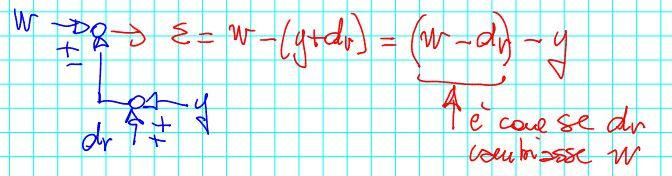
\includegraphics[height=3cm]{../lezione18/img3.JPG}
\end{center}
dove ricordiamo che $\epsilon$ è diverso dall'errore $w-y$ e vale:
\[
    \epsilon = w - (y+d_r) = (w-d_r) - y
\]
da cui vediamo che $d_r$ influisce direttametne su $w$.\newline
\newline
Riassumendo:\newline
$Y= \frac{Y}{W} \cdot  W + \frac{Y}{D_a} \cdot  D_a + \frac{Y}{D_r} \cdot D_r = TW + SD_a - TD_r$, perchè $T = \frac{Y}{W}$ e $S= \frac{Y}{D_a}$ e $-T = \frac{Y}{D_r}$.\newline
Notiamo che nell'espressione precedente nel termine, per esempio, $\frac{Y}{W} \cdot  W$, non si semplificano le $W$, perchè $\frac{Y}{W}$ va interpretato come "$\frac{\text{EFFETTO di $W$ su "Y"}}{W}$", cioè $\frac{\mathcal{L}[Y_F]}{\mathcal{L}[W]}_{D_a = D_r = 0}$.
\subsection{Requisiti del controllo}
\begin{itemize}
    \item \textbf{Anello chiuso asintoticamente stabile (AS)}.
    \item \textbf{Precisione statica}, cioè che se si impongono ingressi costanti ($w(t) = \bar{w}$, $d_a(t) = \bar{d}_a$, $d_r(t) = 0$), allora, assunto anche il punto precedente, esiste finito il limite $\lim_{t\rightarrow \infty} e(t) = e_{\infty}$, dove $e_\infty$ prende il nome di \textbf{errore a regime}. \newline
    Detto in maniera più semplice possiamo dire che precisione statica significa che presi degli ingressi costanti, a transitorio esaurito, l'errore deve essere piccolo.\newline
    Tipicamente viene richiesto che proprio questo errore a regime sia $e_\infty = 0$ oppure $e_\infty < $ tot.\newline
    \textbf{oss.} questi concetti possono poi essere estesi a segnali canonici.
    \item \textbf{Precisione dinamica}, cioè quando cambio $w$, $y$ lo deve raggiungere "presto e bene", per esempio senza oscillazioni eccessive.
    \item \textbf{Grado di stabilità}. Il sistema deve essere "abbastanza lontano" dal perdere la stabilità asintotica a seguito di variazioni di qualche suo parametro fisico.
    \item \textbf{Moderazione del controllo}. A parità delle altre proprietà è preferibile il controllore che sollecita meno l'attuatore.
\end{itemize}
\newpage
\section{Stabilità asintotica di sistemi retroazionati (SD LTI a TC SISO)}
[immagine dagli appunti del prof]
\begin{center}
    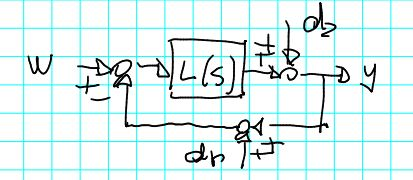
\includegraphics[height=3cm]{../lezione18/img4.JPG}
\end{center}
Poichè la stabilità non dipende dagli ingressi, posso studiare questo schema:\newline
[immagine dagli appunti del prof]
\begin{center}
    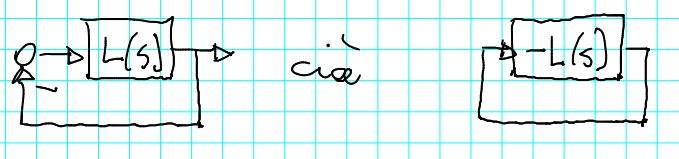
\includegraphics[height=3cm]{../lezione18/img5.JPG}
\end{center}
Posto $L(s) = \frac{L_n(s)}{L_d(s)}$ con $L_n$ e $L_s$ polinomi (cioè, per ora li stiamo considerando senza ritardi), allora definendo $q$ possiamo dire:\newline
[immagine dagli appunti del prof]
\begin{center}
    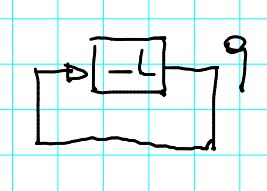
\includegraphics[height=3cm]{../lezione18/img6.JPG}
\end{center}
$-Lq = q$\newline
$q + Lq = 0 \Rightarrow q + \frac{L_n}{L_d}q = 0$\newline
$(1+\frac{L_n}{L_d}) q = 0 \Rightarrow \frac{L_n+L_d}{L_d}q = 0$\newline
da cui ricaviamo che
\[
    L_n + L_d = 0
\]
che prende il nome di \textbf{equazione caratteristica del sistema in anello chiuso (AC)} e le sue radici sono i poli del sistema in AC.\newline
\newline
Ci occorrono quindi criteri per studiare la stabilità asintotica dell'anello \textbf{chiuso} osservando la funzione di trasferimento $L(s)$ dell'anello \textbf{aperto}, perchè, siccome $L = RP$, se trovo una "buona" $\bar{L}$ è immediato calcolare $R = \frac{\bar{L}}{P}$.\newline
\newline
Per farlo vedremo due criteri: \textbf{Nyquist} e \textbf{Bode}.
\subsection{Diagramma di Nyquist}
Definiamo il \textbf{diagramma di Nyquist} di una funzione di trasferimento $G(s)$ come l'immagine secondo $G(s)$ del percorso di Nyquist relativo a $G(s)$.\newline
\newline
Definiamo il \textbf{percorso di Nyquist} come segue:
\begin{center}
    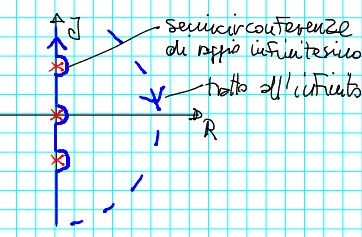
\includegraphics[height=4cm]{../lezione18/img7.JPG}
\end{center}
Si identificano (con le crocette rosse) eventuali poli di $G(s)$ sull'asse $J$. Il percorso è composto dall'asse immaginario percorso dal basso verso l'alto, i poli vengono "schivati" con delle semicirconferenze infinitesime, e il percorso di conclude con una semicirconferenza all'infinito.\newline
\newline
\textbf{oss.} il percorso di Nyquist circonda in senso orario il semipiano destro.\newline
\newline
Poichè $G(-j \omega) = \bar{G}(j \omega)$, il diagramma di Nyquist (DN) è simmetrico rispetto all'asse reale ed è fatto dal percorso di Nyquist completato appunto con tale simmetrico.
\subsubsection{Esempi}
\textbf{es.} \newline
[immagine dagli appunti del prof]
\begin{center}
    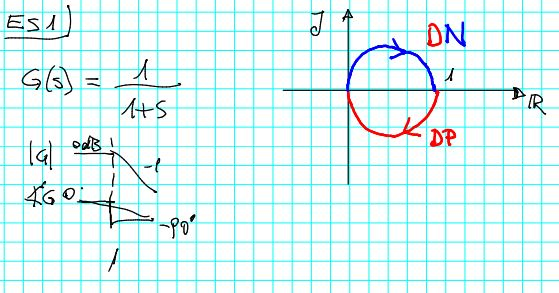
\includegraphics[height=5cm]{../lezione18/img8.JPG}
\end{center}
(diagramam polare in rosso, diagramma di Nyquist in rosso+blu, completato a partire da quello polare con il suo simmetrico)\newline
\rule{\textwidth}{0,4pt}
\textbf{es.} \newline
[immagine dagli appunti del prof]
\begin{center}
    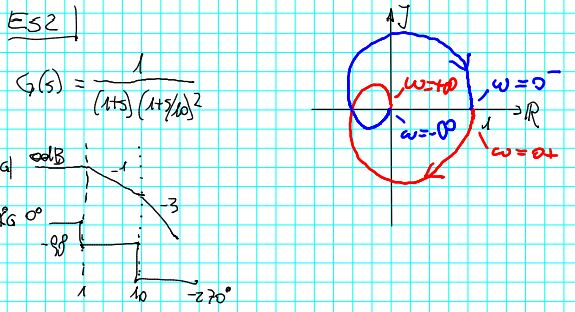
\includegraphics[height=5cm]{../lezione18/img9.JPG}
\end{center}
(diagramam polare in rosso, diagramma di Nyquist in rosso+blu, completato a partire da quello polare con il suo simmetrico)\newline
\rule{\textwidth}{0,4pt}
\textbf{es.} \newline
[immagine dagli appunti del prof]
\begin{center}
    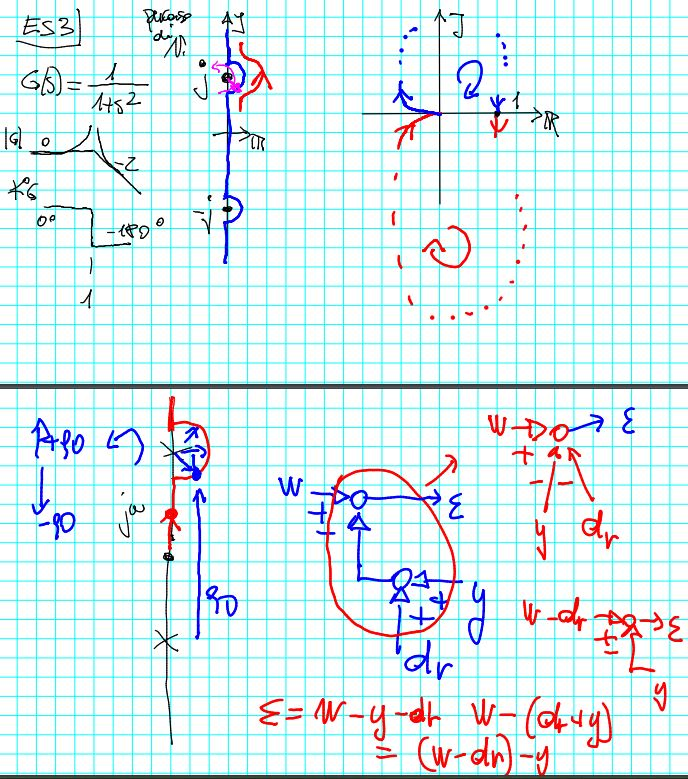
\includegraphics[height=9cm]{../lezione18/img10.JPG}
\end{center}
(diagramam polare in rosso, diagramma di Nyquist in rosso+blu, completato a partire da quello polare con il suo simmetrico).\newline
\newline
Correzione della lezione successiva su questo esercizio:\newline
[immagine dagli appunti del prof]
\begin{center}
    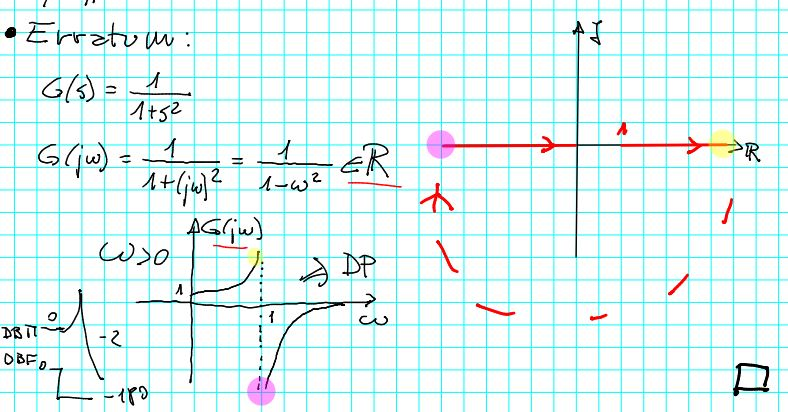
\includegraphics[height=5cm]{../lezione18/img11.JPG}
\end{center}
\rule{\textwidth}{0,4pt} 
